\documentclass[12pt]{article}
\usepackage[utf8x]{inputenc}
\usepackage{hyperref}
\usepackage{amsmath}
\usepackage{graphicx}
\usepackage[colorinlistoftodos]{todonotes}
\usepackage[toc,page]{appendix}
\usepackage{smartdiagram}
\usepackage{indentfirst}


\usetikzlibrary{fit}


\begin{document}
\graphicspath{{images/}}
\begin{titlepage}

\newcommand{\HRule}{\rule{\linewidth}{0.5mm}} % Defines a new command for the horizontal lines, change thickness here
\setlength{\topmargin}{0in}
\center % Center everything on the page


 \begin{minipage}{0.4\textwidth}
\begin{flushleft} \large
\hspace*{-0.5cm}

\includegraphics[scale=0.4]{images/imag.jpg}\\
\end{flushleft}
\end{minipage}
~
\begin{minipage}{0.5\textwidth}
\begin{flushright} \large
\hspace*{2cm}

\includegraphics[scale=0.4]{images/company.png}\\
\end{flushright}
\end{minipage}\\[1cm]
%----------------------------------------------------------------------------------------
%	HEADING SECTIONS
%----------------------------------------------------------------------------------------

\textsc{\LARGE Université Grenoble Alpes}\\[1.5cm]
\textsc{\Large Master 2 Génie Informatique}\\[0.5cm]
\textsc{\large Mémoire d'Alternance}\\[0.5cm]

%----------------------------------------------------------------------------------------
%	TITLE SECTION
%----------------------------------------------------------------------------------------

\HRule \\[0.4cm]
{ \huge \bfseries Ingénieur DevOps}\\[0.4cm]
\HRule \\[1cm]

%----------------------------------------------------------------------------------------
%	AUTHOR SECTION
%----------------------------------------------------------------------------------------

\begin{minipage}{0.4\textwidth}
\begin{flushleft} \large
\emph{Author:}\\
Gerardo \textsc{LARREINEGABE} \\
\end{flushleft}
\end{minipage}
~
\begin{minipage}{0.5\textwidth}
\begin{flushright} \large
\emph{Maître d’apprentissage:} \\
Duy \textsc{Tran Quang} \\[0.5cm] % Supervisor's Name
\emph{Tuteur Pédagogique:} \\
Olivier \textsc{Gruber} % Supervisor's Name
\end{flushright}
\end{minipage}\\[1cm]

%----------------------------------------------------------------------------------------
%	DATE SECTION
%----------------------------------------------------------------------------------------

{\large Grenoble, le 25 août 2018}\\[0.5cm]


\vfill % Fill the rest of the page with whitespace

\end{titlepage}

\renewcommand{\abstractname}{Résumé}
\begin{abstract}
\noindent
Dans le cadre de mon alternance, j'ai intégré l'équipe de IT au sein de
la société Bonitasoft, qui gère plusieurs projets dont BCD forme part et vise
à fournir au client une solution DevOps et des bonnes pratiques pour aboutir
à la Livraison Continue des applications créés avec Bonitasoft.
Le nom BCD est l'acronyme en anglais de \textit{Bonita Continuous Delivery}. \\
BCD aborde deux problème commun des développeur qui est la \textbf{création}
d'un environnement normalisé et le \textbf{déploiement} d'une application
Bonitasoft.\\ \\
\textbf{\textit{Mot clés:} livraison continue, déploiement,
création d’environnement, devops}
\end{abstract}

\newpage
\tableofcontents
\newpage

\section{Introduction}
Dans le cadre de mon alternance, j'ai occupé un poste d'Ingénieur DevOps dans
l'entreprise Bonitasoft.
Pour commencer, je présenterai mon entreprise, l'organisation, les différentes équipes,
la méthode de travail de façon générale.
En deuxième partie, je mettrai un accent sur l'équipe avec laquelle j'ai collaboré,
l'organisation interne, la façon de travailler et les activités que l'équipe
mène tous les jours.
En troisième, j'exposerai le projet sur lequel j'ai travaillé, la problématique,
et les objectifs de mon sujet, ainsi que les différentes techniques requises pour
les accomplir.

\section{Environnement Professionnel}
\subsection{L'entreprise}
\subsubsection{Mission-Vision}
De la démocratisation du BPM à la transformation numérique en profondeur de l'entreprise, nous sommes à la pointe d'une révolution professionnelle depuis que notre entreprise a vu le jour.
Le succès de nos clients est notre succès, et tout le monde chez Bonitasoft est un contributeur, chaque jour.
\cite{Bonitasoft2017BONITA1}

\subsection{Un peu d'Histoire}
Bonitasoft est un éditeur de logiciel open source créé en 2001. Il a commencé comme
Bonita BPM dans l'Institut National de Recherche en Informatique et en
Automatique (INRIA) puis transféré au Groupe Bull.
En 2009, Miguel Valdés Faura rejoint Charles Souillard et Rodrigue Le Gall pour
fonder Bonitasoft.
En 2011, après une série de levée de fonds, Bonitasoft a pu commercialiser son
produit Bonita à l'international et le premier bureau de Bonitasoft est ouvert
aux Etats-Unis.\cite{wikipedia_2018}



\subsection{Organisation}
Bonitasoft a quatre bureaux principaux, aux États-Unis, à San Francisco et à New York,
en France à Paris et à Grenoble.
Les activités sont organisée et divisée en 5 different services:


\begin{center}
  \smartdiagramset{bubble node size=4cm, bubble center node size=6cm}
  \smartdiagram[bubble diagram]{Bonitasoft,
  IT,Service Professionnel,
  R\&D, Support, Succès du Client}
\end{center}


\subsubsection{IT}
Le département de l'IT est le gardian principal de tout le tâches IT commun comme:
\begin{itemize}
  \item La gestion des environnements virtuels. (cloud ou serveur physique).
  \item La gestion de l'automatisation de processus de CI interne.
  \item La gestion des licences des applications payent (OS, applications).
  \item La gestion des appareils, périphériques, les ordinateurs portables,
  \item L'architectures, méthodologies et règles régissant l'utilisation et le stockage des données.
  \item L'administration de systèmes: la configuration, gestion, entretien et dépanne des environnement
  informatique multi-utilisateur (cloud ou physique).
  \item  La gestion ou l'aide aux autres département avec la culture et pratiques DevOps.
\end{itemize}

Aussi, l'équipe d'IT de Bonitasoft gère d'autres projets comme:
\begin{itemize}
  \item Salesforce: depuis la création des use cases jusqu'à la mise en production en garantissant la gouvernance du système avec une approche DevOps.
  \item BCD: c'est une solution fournit pour utiliser les bonnes pratiques DevOps pour la livraison continue (CI) d'une application Bonita.
\end{itemize}

L'équipe est composée de quatre personnes, dont l'une est moi.

\begin{figure}[h]
  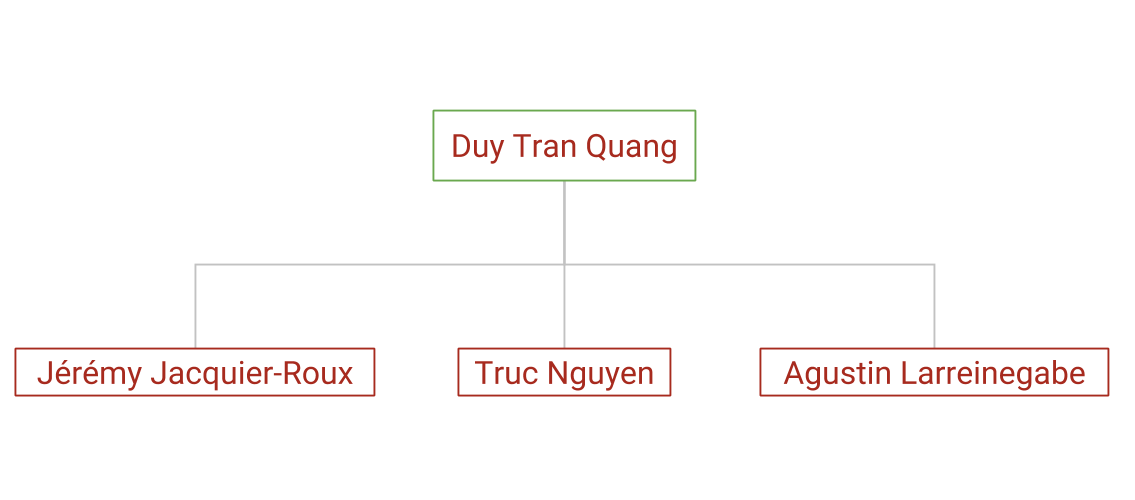
\includegraphics[width=\textwidth,keepaspectratio]{it_team.png}
   \caption{Organigramme.}
   \label{figure:organigrame}
\end{figure}

\subsubsection{R\&D}
Il est le plus grand département et son travail principal est le développement de la plate-forme Bonitasoft.
Il est divisé par équipes de travail ou projets:
\begin{itemize}
  \item Back-end
  \item Front-end
  \item BICI, c'est une application autonome connectée au moteur de Bonita qui permet d'analyser l'exécution
   des processus et prévoir et améliorer l'efficacité de l'équipe.
\end{itemize}

\subsubsection{Customer Success (CS)}
Le département gère la relation entre Bonitasoft et ses clients. L'objectif de la réussite du client est de rendre le client le plus performant possible, ce qui, à son tour, améliore la valeur à vie du client pour l'entreprise.
Cette fonction est la plus couramment utilisée dans le monde du logiciel et la plus répandue parmi les sociétés de services. Parce que le succès du client est un domaine naissant, son alignement organisationnel et ses activités sont toujours en évolution.

\subsubsection{Support}
Ce département est en charge de traiter et de diriger les différentes questions et problématiques du client.
Chaque problème ou bogue est chargé dans l'outil Jira et traité par le département R\&D ou l'IT.
Chaque ticket chargé a une priorité et il est résolu par ordre de priorité.

\subsubsection{Service Professionnel}
C'est une équipe d'experts qui offre de la valeur pour le succès du client en suivant les projets depuis le début avec la meilleure expérience-utilisateur possible.



\section{Produits} \label{produits}
Actuellment, l'entreprise a une produit principal qui est \emph{Bonita}, et deux produits complémentaire qui sont \textit{Bonita Continuous Delivery} et \textit{Bonita Intelligent Continuous Improvement}

Dans cette partie, nous allons introduire de manière superficiel tous les produits pour avoir un contexte plus claire de la mission.

\begin{figure}[!ht]
\centering
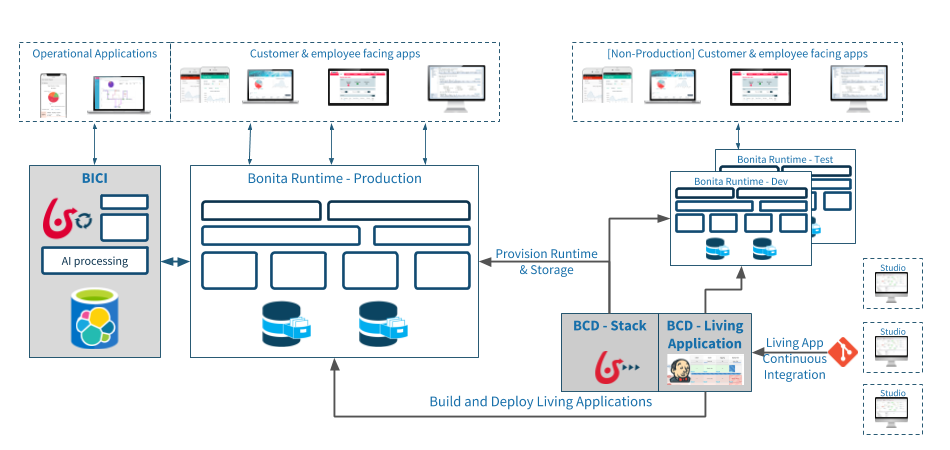
\includegraphics[scale=0.39]{bonita_add-on_archi.png}
\caption{Interaction entre Produits}
\label{fig:bonita_add-on}
\end{figure}

\subsection{Bonita}
\begin{quotation}
Le BPM est la discipline de la gestion des processus (plutôt que des tâches) en tant que moyen d'améliorer les résultats de performance de l'entreprise et l'agilité opérationnelle. \cite{gartnerdic}
\end{quotation}

Bonita est une plate-forme basé sur BPM qui sert à construire des applications, personnalisées, en prenant l'avantage plein du BPM pour s'adapter aux changements en temps réel.

La plate-forme a deux parties. Voir Figure \ref{fig:bonita_archi}:
\begin{itemize}
  \item Bonita Studio
  \item Bonita Plate-forme (Bonita Engine)
\end{itemize}

\subsubsection{Bonita Studio}
Bonita le Studio est un environnement graphique pour créer des processus, des applications, des modèles de données et des vues d'utilisateurs. Il contient trois outils de design(conception) majeurs:

\begin{itemize}
  \item Le tableau blanc, pour dessiner un organigramme de processus et définir les transitions.
  \item Le menu de Développement, pour étendre les capacités du Studio et crée les modèles de données.
  \item Le Concepteur UI, qui est utilisé pour créer des pages d'application et des formulaires de processus
\end{itemize}

Le Studio contient une Plate-forme Bonita (Tomcat, UI Designer, Bonita Portal, Bonita Engine et une base de données H2), approprié pour tester une application

\subsubsection{Bonita Engine}
C'est le runtime processeur au cœur de Bonita. Il exécute des processus, en traitant des actions liées aux tâches, comme l'accès de base de données. Le Moteur est composé d'un certain nombre de services et API. Les services sont services BPM ou des services génériques.

\begin{figure}[!ht]
\centering
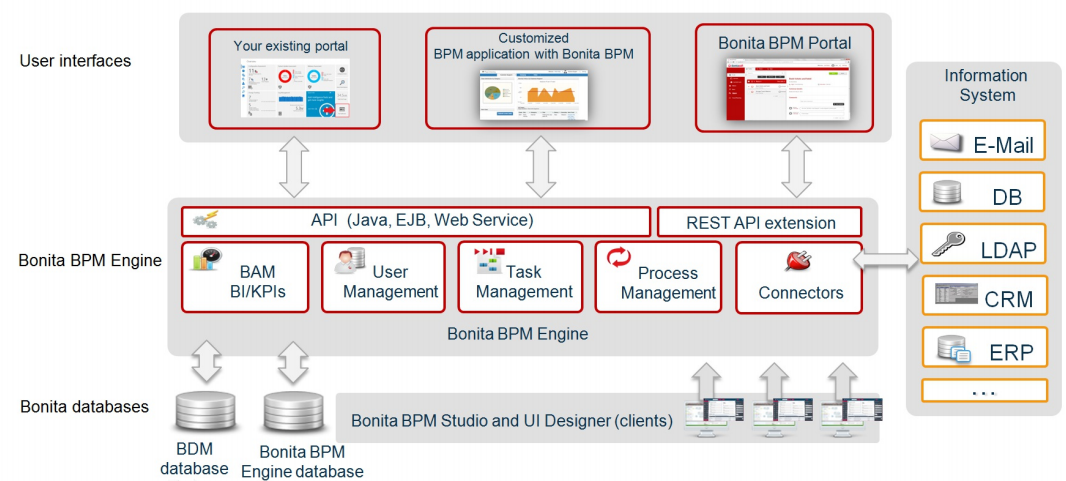
\includegraphics[scale=0.5]{bonita_archi.png}
\caption{Bonita Architecture}
\label{fig:bonita_archi}
\end{figure}

\subsection{Bonita Continuous Delivery (BCD)} \label{bcd}
Bonita Continuos Delivery ou \textit{BCD} est une solution qui permet l'intégration continue d'une application Bonita en promouvant aussi des bonnes pratiques \emph{DevOps}

Au début, BCD a démarré à partir d'un besoin interne de tester plus facilement des développements. La mise en place d'un environnement avec l'installation de \textit{Bonita Engine} était un processus lent et répétitif, aussi, suite à divers retours des clients, la Directive a décidé de voir comme un potentiel produit.

Actuellement, \textit{BCD} a deux parties. Voir Figure \ref{fig:bcd_cap}:
\begin{itemize}
  \item Livingapp, qui permet la compilation d'un projet avec la gestion de bibliothèques essentielles pour une application \textit{Bonita Subscription}, sans avoir besoin de Bonita Studio, et aussi de déployer l'application compilé dans un stack Bonita configuré.
  \item Stack, qui permet d'un part la création des environnements virtuels dans le cloud (AWS actuellement), et l’installation d'un Stack Bonita dans les serveurs configurés.
\end{itemize}

\begin{figure}[!ht]
\centering
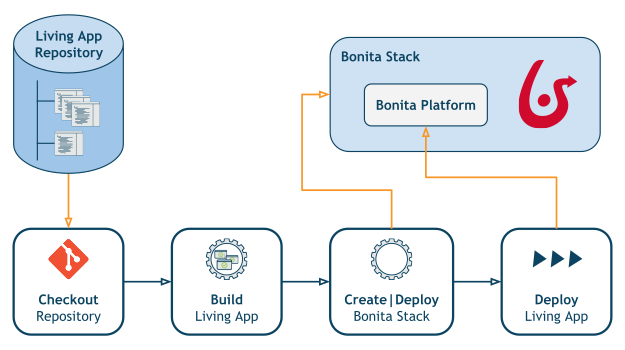
\includegraphics[width=\textwidth,keepaspectratio]{bcd_capabilities.png}
\caption{Fonctionnalités BCD}
\label{fig:bcd_cap}
\end{figure}

\subsection{Intelligent Continuous Improvement (ICI)}

ESCRIBIR


\section{Devops}
\subsection{Culture}
Nowadays, in digital business, we offer and delivery wide range of services through digital experiences and to improve these services we have to have the feedback from the customer to start being able to deliver new types of experiences and values. Doing this, we are going to be more competitive and interact with the customer in new ways, something that all industries are going through.
All these, we can arrive just doing with good practices to do the work far far more efficient. Here we enter in the DevOps World.

DevOps is primely  about the culture, collaborative practices and automation that aligns Development and Operation teams so that they have a single mindset on improving customer experiences, responding faster to business needs, and ensuring that innovation is balanced with security and operational needs \cite{IsaacSacolick2016DrivingCulture}. This means:

\begin{itemize}
\item Automate testing.
\item Ensure more frequent and reliable deployments.
\item Develop clarity on roles and responsibilities.
\item Define Key Performance Indicator \(KPI\) and scopes.
\item Automating and monitoring.
\end{itemize}

To start this concept, we have to make sure the people are aligned with what DevOps is, and with a challenge and not with the whole set of DevOps practices.

Also, we have to keep the focus in QA knowing that it is a distinct discipline and skill set, but should work with Dev to develop and automate test case.

\paragraph{Participant}
% https://youtu.be/eMSrjr5vyoI 24min PARTe de organizacion 
\subparagraph{Dev}
QUe es Dev y q deberia hacer
%https://youtu.be/q01IjipC-8o Digital Driving

\subparagraph{Ops}
QUe es Ops y q deberia hacer

\subsection{Continues everyone}
%https://youtu.be/oGX8DB9aZb0
no podemos automanizar todo, como devops es tambien una cultura, y cultura incluye a las personas, no podemos automatizar a las personas.
Son las personas 


\section{Réflexion final}
Cette formation en alternance m'a permi d'obtenir beaucoup de compétences et des
savoir-faire que ce soit sur le plan informatique avec la multitude de nouvelles
technologies abordées s'ajoutant aux connaissances déjà acquises que j'ai pu
approfondir. Mais également sur le plan personnel, toute la confiance qui m'a
été donnée dès mon arrivée par l'équipe, ma liberté d'expression et de prise de
décisions ainsi que le partage d'expériences avec les collegues on été très
enrichissants et formateurs.

\subsubsection{Bilan professionnel}

\subsubsection{Bilan personnel}


\subsection{Challenges}
blabla

\subsection{Skills and Teachings}
blabla

\subsection{Skills and Teachings}
blabla

\subsection{Future Work}
blabla


\section{Conclusion}
Cette expérience a été passionnante et enrichissante d'une part, grâce à l'équipe humaine qui donne tout son potentiel tous les jours, et pas seulement pour être efficace dans le travail, mais aussi pour construire une ambiance de croissance, d'amélioration et de support.
D'autre part, parce que grâce à la mission, j'ai pu approfondir mes connaissances sur la culture DevOps, ses enjeux, sa difficulté et ses bénéficies.

\section{Remerciements}
Pour clore mon rapport, je souhaiterais adresser mes remerciements en premier à ma famille et à ma copine qui m'ont toujours apporté leur soutien, ainsi qu’au Programme BECAL pour son financement et la confiance qui m'a été donnée pendant deux ans.

Je tiens aussi à remercier toute l'équipe avec laquelle j'ai eu le plaisir de travailler :
\begin{itemize}
  \item[] mon maître de stage Duy Trang Quang pour m’avoir toujours fait confiance,
  \item[] Jérémy Jacquier-Roux pour son amitié et ses conseils,
  \item[] Truc Nguyen pour sa rigueur.
\end{itemize}
Ils sont toujours été à l'écoute lorsque j'avais une question ou une proposition.

Je remercie également mon tuteur Olivier Gruber pour le temps qu’il m’a consacré cette année et pour tous les conseils qu’il m’a donnés.

Je tiens finalement à remercier tous mes collègues de Bonitasoft pour leur convivialité, pour l’ouverture et l'esprit d'amélioration continue qu’ils ont partagés avec moi cette année.





\newpage
\addcontentsline{toc}{section}{Références}
\newpage

\begin{appendices}
\section{Back log}
Jira Backlog

\newpage
\section{Contribution}
GITHUB
\end{appendices}
\textbf{}
\bibliographystyle{plain}
\bibliography{reportbiblio}
\end{document}
